\documentclass[border=10pt]{standalone}
\usepackage{pgfplots}
\pgfplotsset{compat=1.18}
\usepgfplotslibrary{colormaps}

\begin{document}
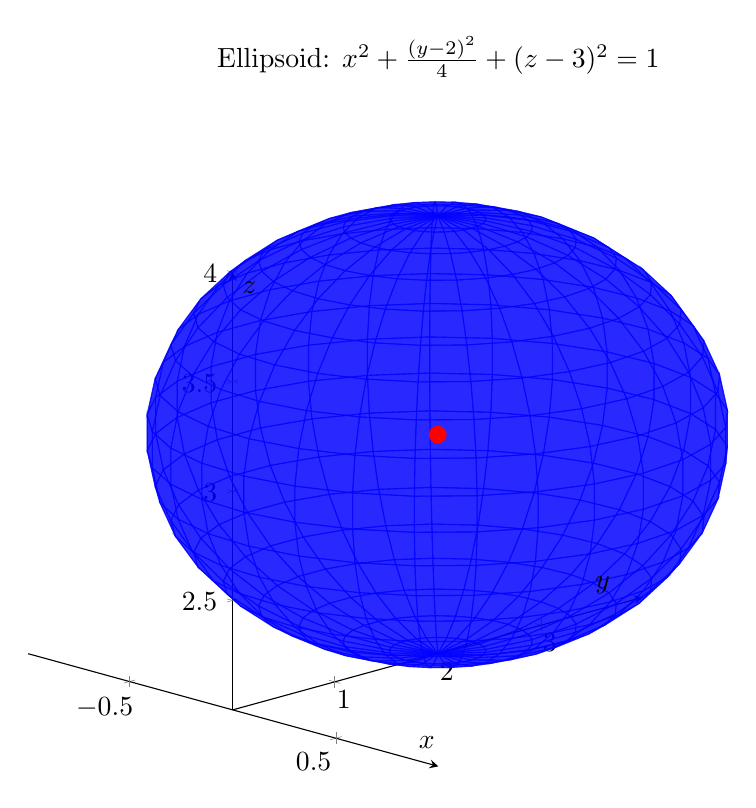
\begin{tikzpicture}
\begin{axis}[
    width=12cm,
    height=10cm,
    xlabel={$x$},
    ylabel={$y$},
    zlabel={$z$},
    title={Ellipsoid: $x^2 + \frac{(y-2)^2}{4} + (z-3)^2 = 1$},
    view={45}{20},
    axis lines=center,
    grid=major,
    colormap/viridis,
    z buffer=sort,
]

% Parametric ellipsoid surface
% x = cos(u)*sin(v), y = 2 + 2*sin(u)*sin(v), z = 3 + cos(v)
\addplot3[
    surf,
    opacity=0.6,
    shader=flat,
    domain=0:360,
    y domain=0:180,
    samples=30,
    samples y=20,
    blue
] ({cos(x)*sin(y)}, {2 + 2*sin(x)*sin(y)}, {3 + cos(y)});

% Center point
\addplot3[
    only marks,
    mark=*,
    mark size=3pt,
    red
] coordinates {(0, 2, 3)};

\end{axis}
\end{tikzpicture}
\end{document}